\section{The Neocortex}
What separates all mammals from the rest of the animal kingdom is the existence of the neocortex in the cerebral cortex \cite{Neocortex}. The neocortex is perceived as the part of the brain where intelligence resides. The reason for this is that the neocortex is responsible for higher order brain functions, such as sensory perception, advanced motor control, association, memory, and cognition \cite{LodatoSimona2015GNDi}.  



\begin{figure}[ht!]
    \centering
    \begin{tikzpicture}
        \node[anchor=south west,inner sep=0] (image) at (0,0)
        {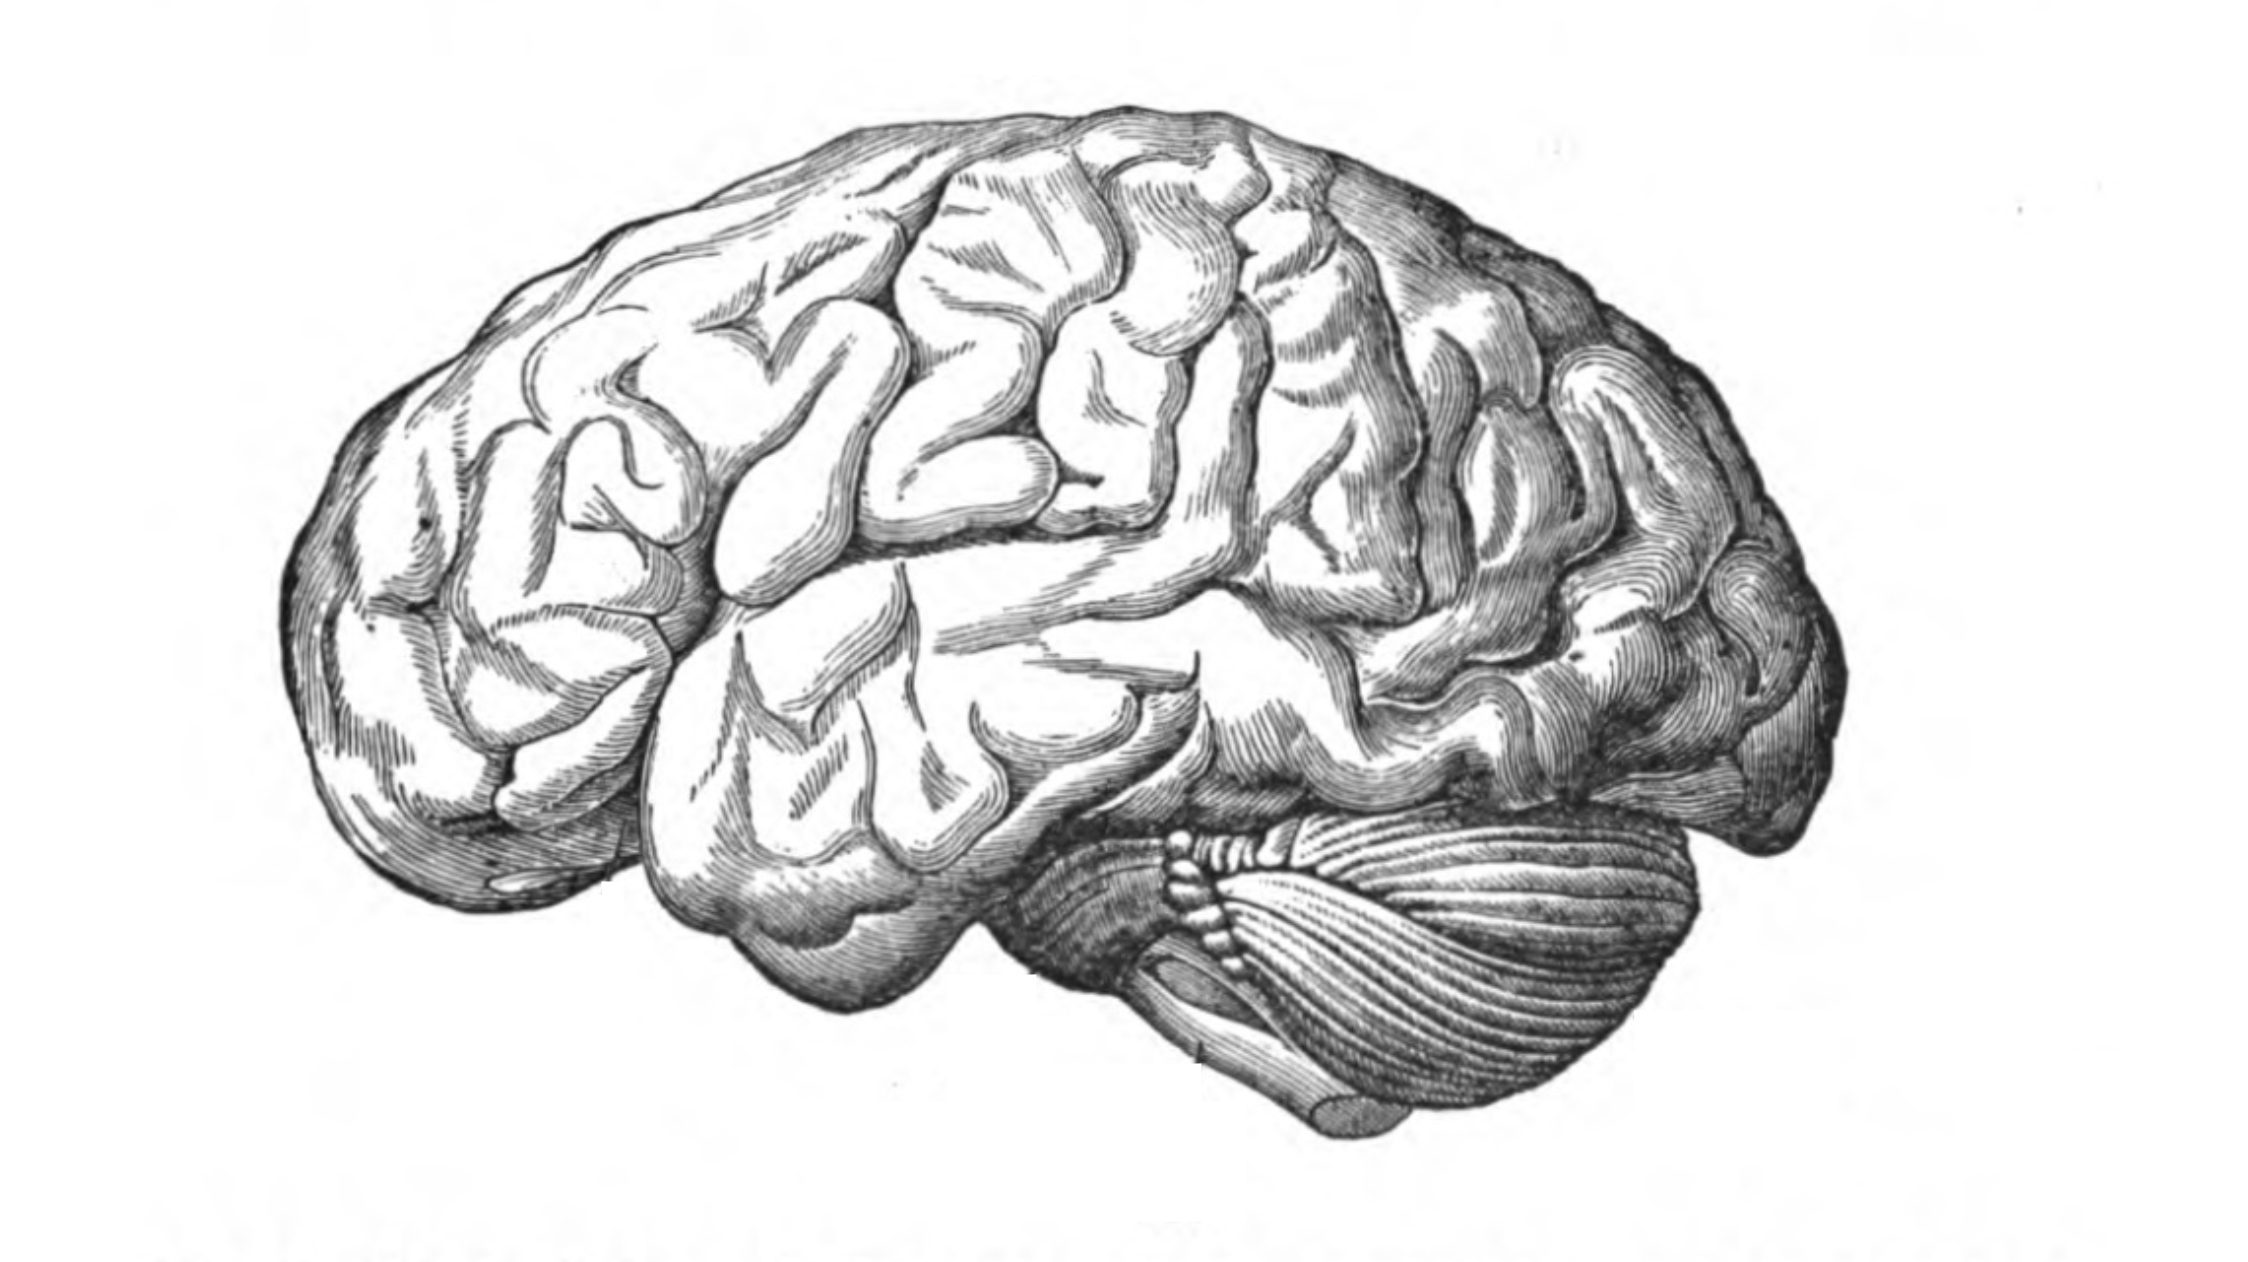
\includegraphics[scale=.35]{appendix/neuroscience/figures/brain2.png}};
        \node [anchor=west] (Neocortex) at (1,7) {Neocortex};
        \node [anchor=west] (Old Brain) at (3,1) {Old Brain};
            \begin{scope}[x={(image.south east)},y={(image.north west)}]
                \draw [-latex, thick, black] (Neocortex) to[out=0, in=120] (0.45,0.91);
                \draw [-latex, thick, black] (Old Brain) to[out=0, in=-120] (0.6,0.1);
            \end{scope}
    \end{tikzpicture}%
    \caption{\cite{BrainSketch} A sketch of the brain of a Homo sapiens. The cerebral hemisphere is recognised by the convoluted form with ridges and furrows.}
    \label{fig:forebrain}
\end{figure}


The forebrain, shown in figure \autoref{fig:forebrain}, is the largest part of the mammalian brain, made up of the cerebrum, thalamus, and hypothalamus. The cerebrum is made up of two cerebral hemispheres. The cerebral hemisphere has an outer layer of grey matter and the cerebral cortex beneath it \cite{crossman2014neuroanatomy}. The cerebral cortex consists of two areas, the neocortex and the allocortex, defined by their cytoarchitecture \cite{Allocortex}. The neocortex is larger in area and it is the outer most layer of the cerebral cortex, organised into six horizontal laminae of neurons. The allocortex is smaller in size with subareas such as the hippocampus, subiculum and olfactory cortex \cite{Neocortex}. Because mammals share the same brain structure of the olfactory cortex and the hippocampus with reptiles but not the neocortex, it was long viewed that the neocortex was a new evolutionary addition of the brain, hence the name. However, the neocortex should instead be viewed as homologous with the dorsal cortex of reptiles. Though, the difference between them is noticeable, the neocortex is a thick, laminated and uniform structure containing abundance of neurons; compared to the dorsal cortex in reptiles which contains only about a row of neurons in its sheet of tissue \cite{Neocortex}. With these dissimilarities in mind, the function of all vertebrate brains is still the same, which is to act as a premotor organ that sends motor commands to the animals' muscles \cite{10.3389/fnana.2013.00051}. 


What makes the human neocortex so special that its able to give us humans the ability to express our thoughts through motor commands, e.g. writing or speaking, perception, imagination, language processing and cognition? One major factor to why humans surpasses it counterparts in intelligence is the sheer size of the neocortex, a surface area of roughly 2600 cm$^2$ and a thickness of 3-4 mm, together with the vast number of neurons, up to $28\times10^9$, that resides there \cite{MountcastleVernon1997}. The human neocortex wraps around the forebrain in a convoluted fashion, compared to a rodents' neocortex which is non-folded. This allows the human neocortex to have more surface area with a limited volume \cite{folded}. Another reason why humans surpasses all other mammals is evolutionary, i.e. having a large neocortex with many subdivisions is metabolically costly, takes a long time to develop and mature and is unnecessary for most other animals \cite{Neocortex}. 


\subsection{The Topology}
The neocortex organized in hierarchy of six horizontal stacked laminae, numbered I--VI, with each of the layers grouped based on synaptical connectivity, morphological type of neurons and at which depth they exist \cite{Neocortex}. This basic structure is shown in \autoref{fig:layers}. To understand the difference of each layers' topology and processing properties, a brief description is given below:



\begin{itemize}[leftmargin=4em,align=left]
    \item \textbf{Layer I:} The top layer, which is mostly inhabited by fibers that run parallel to the surface. The fibers consist of the ends of apical dendrites and axons that connect to each other via synapses, together with a few neurons. This layer serves two purposes; first, to work as a feedback connection from other cortical areas. Secondly, to modulate input from the brain stem \cite{Neocortex}.
    
    \item\textbf{Layer II:} This layer has a large population of small neurons. The dendrites of these neurons are connected to neighbouring cortical areas and pyramidal neurons in deeper layers via their apical dendrites. Thus, allowing intracortical connections to affect the processing in a local area \cite{Neocortex}.
    
    \item\textbf{Layer III:} One of the main output layers of the neocortex, consisting of medium sized pyramidal neurons with basal and apical dendrites. The axons of these neurons serves as commissural fibers, i.e. connections between the two cortical hemispheres, and as connections to other cortical areas \cite{crossman2014neuroanatomy}. The pyramidal neurons receive their input form other layers in the local area via their apical dendrites. Adjacent neurons in layer III are able exchange information via their basal dendrites. This layer is of great importance, as it makes it possible for information exchange between regions in the neocortex. Thus increasing the complexity of possible operations that can be performed \cite{Neocortex}.
    
    \item\textbf{Layer IV:} The main input layer and situated in the middle occupied by small stellate cells. The name is given due to the radial propagation of the dendrites. The information that the stellate cells receives is shared locally between neighbours via the basal dendrites and then transmitted to the adjoining layers above and below. The stellate cells are small due to the fact that the axons and dendrites only extend a short range \cite{Neocortex}.
    
    
    \item\textbf{Layer V:} This is the other main output layer of the neocortex. Large pyramidal neurons inhabit this layer, which can be seen in \autoref{fig:layers} as triangular black spots. The main task of this layer is to integrate information from both its horizontal neighbours and all vertically connected neurons in the layers above up till layer I that belongs to the same cortical column \cite{Neocortex}. This information is then sent out to extra-cortical parts of the brain, i.e. basal ganglia, thalamus, brain stem and the spinal cord, via long axons \cite{crossman2014neuroanatomy}. But also to remote cortical areas, including areas in the other cerebral hemisphere. As these distances can be quite far and information needs to travel fast, the axons needs thick, as this allows for faster conduction rates. To gather information from the vertically adjoining layers, the apical dendrites branch out in long vertical fibers, with synaptic connections in each layer. Neighbouring cells communicate via their basal dendrites. For the pyramidal neurons to be able to send and receive action potentials on their long apical dendrites, and also thick axons the cell body needs to be large \cite{Neocortex}.
    
    
    \item\textbf{Layer VI:} Until this layer, the information has just been processed in a feed-forward manner, i.e. receive information, manipulate it and transmit it onward to other regions. But bi-directional communication is necessary in any complex computational unit, and this is where layer VI comes in. This is the main feedback layer to other activation regions about the state of the local area. The pyramidal neurons that resides in layer VI mainly get their input for layer IV, as well as direct input from axons that terminate in layer IV. With these connections, layer VI is able to project back information to the neurons in another cortical area that contributed to the activation \cite{Neocortex}. 
    
    
\end{itemize}

\begin{figure}[H]
    \centering
    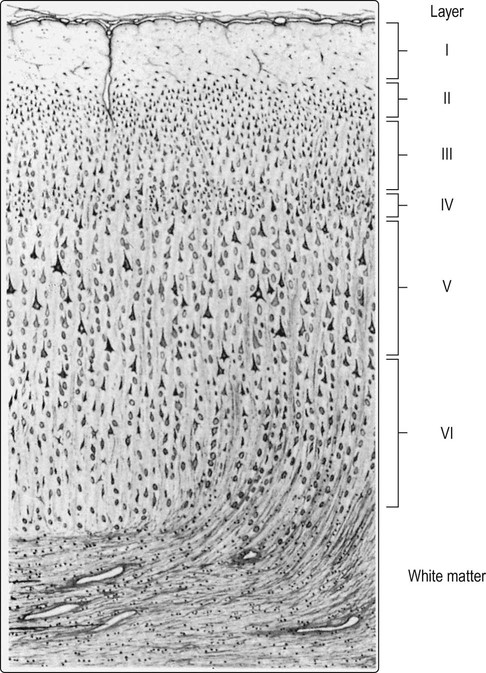
\includegraphics[scale=.88]{appendix/neuroscience/figures/layers.jpg}
    \caption{\cite{IVIlayers} The cross section above, visualises the general structure of the neocortex categorised into six horizontal laminae, I--VI, on the basis of cytoarchitecture. The cell bodies of the neurons are shown as the darkened spots, neither the axons nor dendrites of the neurons are visible. The white matter connects the neocortical region to other regions in the neocortex along with other parts of the brain. These connections allows the region to send and receive signals \cite{Neocortex}.}
    \label{fig:layers}
\end{figure}

\noindent With the understanding of each layers' properties we can now move on to explain the most basic processing unit of the neocortex, the \textit{minicolumn} and the \textit{cortical column}.

%COLUMNAR ORGANISATION
\subsection{Columnar Organisation}
The most basic processing unit in the neocortex is called a \textit{minicolumn}, first described by Vernon B. Mountcastle in 1955--1959 \cite{doi:10.1093/cercor/13.1.2}. A minicolumn is a vertical array of neurons connected to each other like a chain across layer II--VI. These minicolumns have transverse diameter of 50--80 $\mu$m and contain between 80--100 neurons in primates, but can contain up to 2 times more in the striate cortex. The structure of the minicolumn can be observed throughout the neocortex, however they are not identical as some features differ, e.g. cell phenotypes, synaptic transmitters \cite{doi:10.1093/cercor/13.1.2}. A \textit{cortical column} is a group of minicolumns which is formed by a common input and the horizontal links they have with each other. The number of minicolumns that a cortical column contains varies between 50--80 \cite{doi:10.1093/cercor/13.1.2}. The cortical column functions as a complex distributed system, where each minicolumn can be viewed as a computing node, which is able to modulate inputs and use bilateral communication with neighbouring minicolumns and cortical columns. This allows the cortical columns to link multiple inputs to multiple outputs \cite{MountcastleVernon1997}.


\subsection{Neural Circuit Functionality}
In each minicolumn there exists two types of neurons; the \textit{excitatory neurons}, i.e. pyramidal and spiny stellate cells; and the \textit{inhibitory neuron}, the aspiny stellate cells. The neurons are distributed throughout the layers in the minicolumn with the majority, $\sim$80\% , of the neurons being of the excitatory type \cite{Neocortex}. The excitatory neurons are able to depolarise the neurons of which it is synaptically connected to by sending out a excitatory neurotransmitter, glutamate. In this depolarised state the effected neuron is more likely to itself send out an action potential if it receives strong enough signal on its dendrites \cite{Neocortex}. The opposite is true for the inhibitory neuron, as it sends out an inhibitory neurontransmitter, i.e. a biochemical called \textit{gamma-Aminobutyric acid}, or GABA, which hyper-polarises the effected neuron, making it less likely to produce an action potential. This inhibitory effect allows a local circuit to remain sparse, as minicolumns that respond to the same input tend to inhibit each other. This limits the response time for an input and makes the cortical column sensitive to temporal changes \cite{Neocortex}. 


 The cortical columns are able to correlate different inputs based on interconnections that exist in layer III, as these makes horizontal connection in between cortical columns. The advantage of such connections are that neurons in different cortical columns can become active at the same time, thus being able to respond to the signal of the same object and giving it cohesion \cite{Neocortex}. Another crucial part of the neural circuits is its plasticity. The synaptic connections between neurons change over time, either they become stronger or weaker, which makes the brain able to adapt to new input. This is largely due to the two types of membrane receptors that exist, i.e. the \textit{N-methyl-D-aspartate}, or NMDA, receptor and the non-NMDA receptor. The non-NMDA receptor reacts when glutamate is released, which leads to depolarisation of a neuron. When this happens, the NMDA receptor, which is otherwise blocked by magnesium ions, is unblocked and can pass calcium ions through if another glutamate release occurs in a short amount of time. This leads to a fast succession of action potential being generated by the neuron. Because of this, synaptic strength between the the neurons is increased, which is called long-term potentiation. The opposite is called long-term depression, which means that the neurons does not respond to the same input and their synaptic connections are weakened \cite{Neocortex}. This alteration of the synaptic strength between neurons is also known as Hebbian learning \cite{CapaldiE.John1992TOOB}. 
 
 It is in these synaptic connections that memories are stored. Memories are stored in a sequences and can be recalled auto-associatively. This makes the neocortex robust to noise and incomplete input patterns, as it can auto-complete as input patters as memories are recalled in an ordered sequence. Thus, the neocortex is able to make predictions about the future based on incomplete input \cite{memory}. 